
%\addcontentsline{toc}{chapter}{Anhang}
\cftaddtitleline{toc}{chapter}{Anhang}{}
\pagenumbering{Roman}
\appendix


%\chapter{Ausschreibung Bachelorarbeit}\label{anhang_ausschreibung}
% 
%\includepdf{../ressources/Projektorganisation/Ausschreibung.pdf}
%
%
%\chapter{Projektplanung}  \label{anhang_projektplan} 
%%\includepdf [landscape = true, pages=-] {../ressources/Projektorganisation/PlannungV0.pdf}
%
%\vspace*{\fill}\par
%\pagebreak

%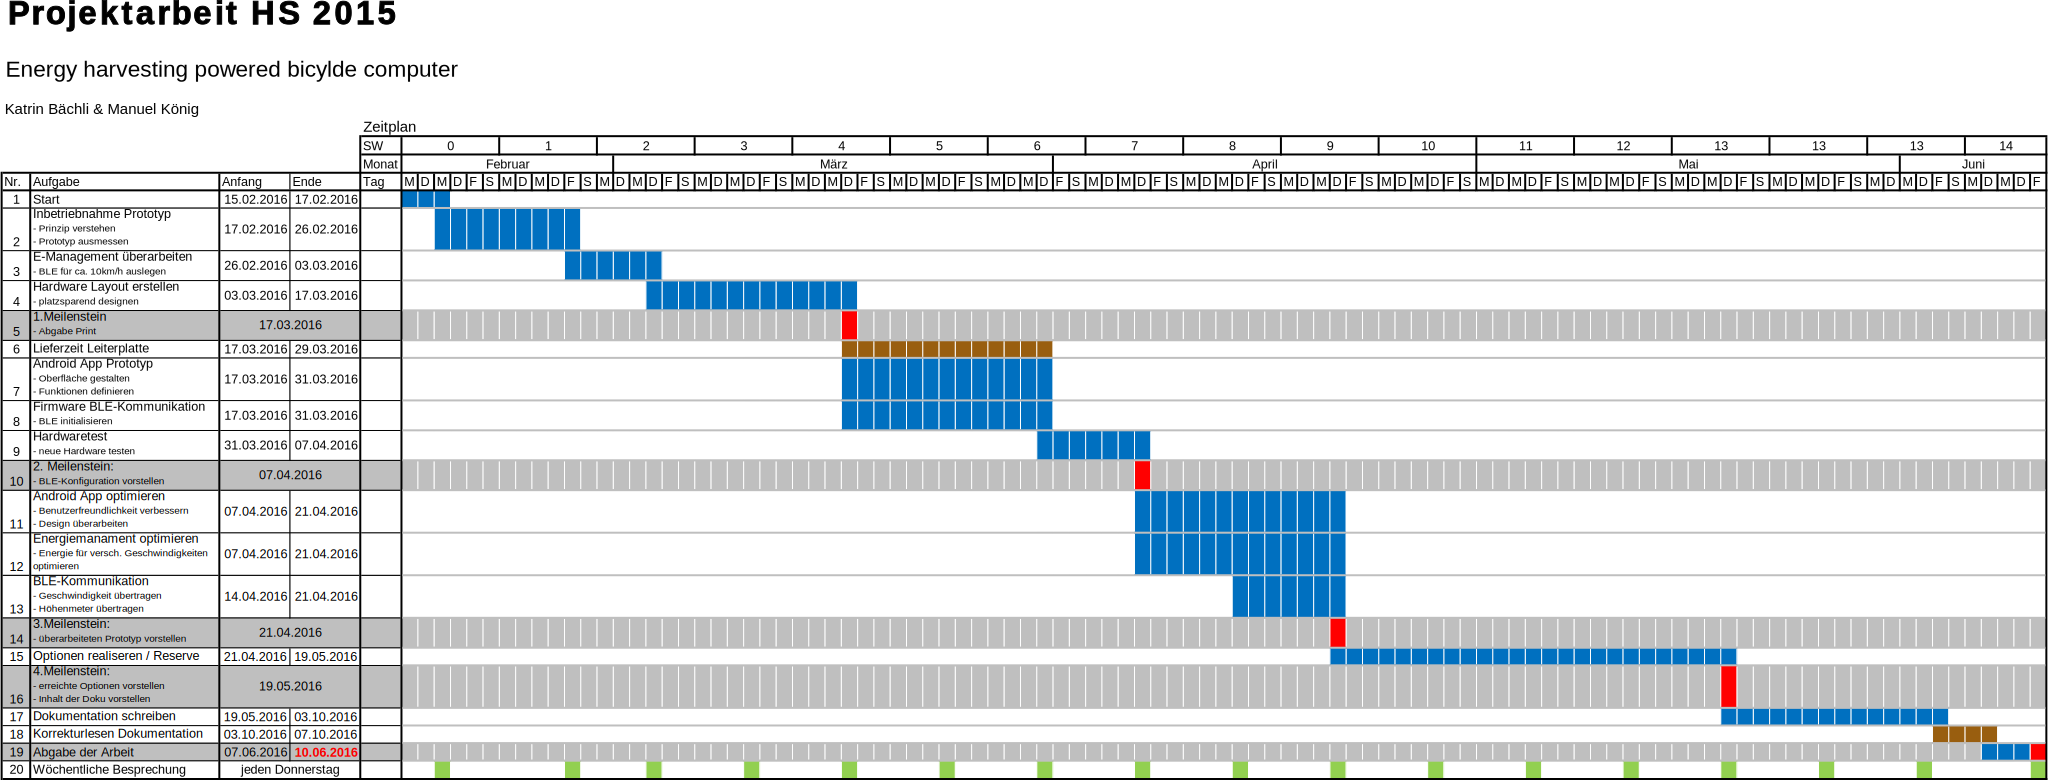
\includegraphics[width=\textheight ,angle=90,origin=c]{../ressources/Projektorganisation/PlannungV0-cropped.pdf}

\chapter{Ausschreibung Bachelorarbeit}

\begin{figure}[h]
    \includegraphics {7Anhang/docs/Ausschreibung.pdf} 
     \caption{Offizielle Ausschreibung der Arbeit}\label{Ausschreibung} 
\end{figure}



\chapter{Blockdiagramm EM8500}\label{anhang_em8500} 
\begin{figure}[h]
    \includegraphics {7Anhang/imag/blockdiagrammEm8500.png} 
     \caption{Blockschema Sensortag}
\end{figure}



\chapter{Funktionsblöcke Sensortag von Texas Instrument}\label{anhang_sensortag} 



\begin{figure}[h]
    \includegraphics {7Anhang/imag/CC26xx_Block_Diagram.png} 
     \caption{Blockschema Sensortag}
\end{figure}

\cite{Sensortag_Datasheet}S.3


%\chapter{Messprotokoll Energiegewinnung Harvester}\label{anhang_messprotokoll_energie_harvester} 
%\includepdf[pages=-]{../ressources/Energiemessungen/MessungHarvesterschaltungV0.pdf}
%
%
%\chapter{Messprotokoll Energieverbrauch Sensortag}\label{anhang_messprotokoll_energie_sensortag} 
%%\includepdf{../ressources/Projektorganisation/Ausschreibung.pdf}
%
%\chapter{Messprotokoll Rippelspannung Ausgangskondensator Harvesterschaltung}\label{anhang_messprotokoll_kondensator_harvester} 
%\includepdf[pages=-]{../ressources/Energiemessungen/MessungKondensatorAusgang.pdf}